\clearpage
\section{Tracking analysis}\label{sec:ana}
Now we have the straws are calibrated with the \num{300 000} events, we want to reconstruct other \num{200 000} events with \verb|StyxM2C2| (of course with calibration applied). The program \verb|StyxLabCourse| is used for the analysis. It contains a class \verb|StudentAnalysis|, where extra code can be inserted to analyze the data. Since the its methods are called for every event, it becomes easier to store some rudimentary histograms to \verb|root| files first and use macro to draw rather complicated histograms.

One can inspect the number of hits for each layer in one module. For example, the plot of bottom module is figure~\ref{fig:hitsLayers}. It is expected that the three histograms have similar shapes, considering there physical vicinity. The shapes originate from the geometry of the detectors: some straws are just longer than others, resulting more hits.
\begin{figure}[ht]
	\centering
	\includegraphics[width=0.8\linewidth]{hitsLayers.pdf}
	\caption{Number of hits per straws for each layer in bottom module}%
	\label{fig:hitsLayers}
\end{figure}

Comparison of total numbers of hits in modules is potentially interesting as well. Figure~\ref{fig:hitsModules} shows the total number of hits in bottom and top modules. They have similar shapes in some regions, but quite different in some other regions. This can be caused by the "qualities" of straws, i.e.~positions of dead and hot straws on the modules don't match each other.
\begin{figure}[H]
	\centering
	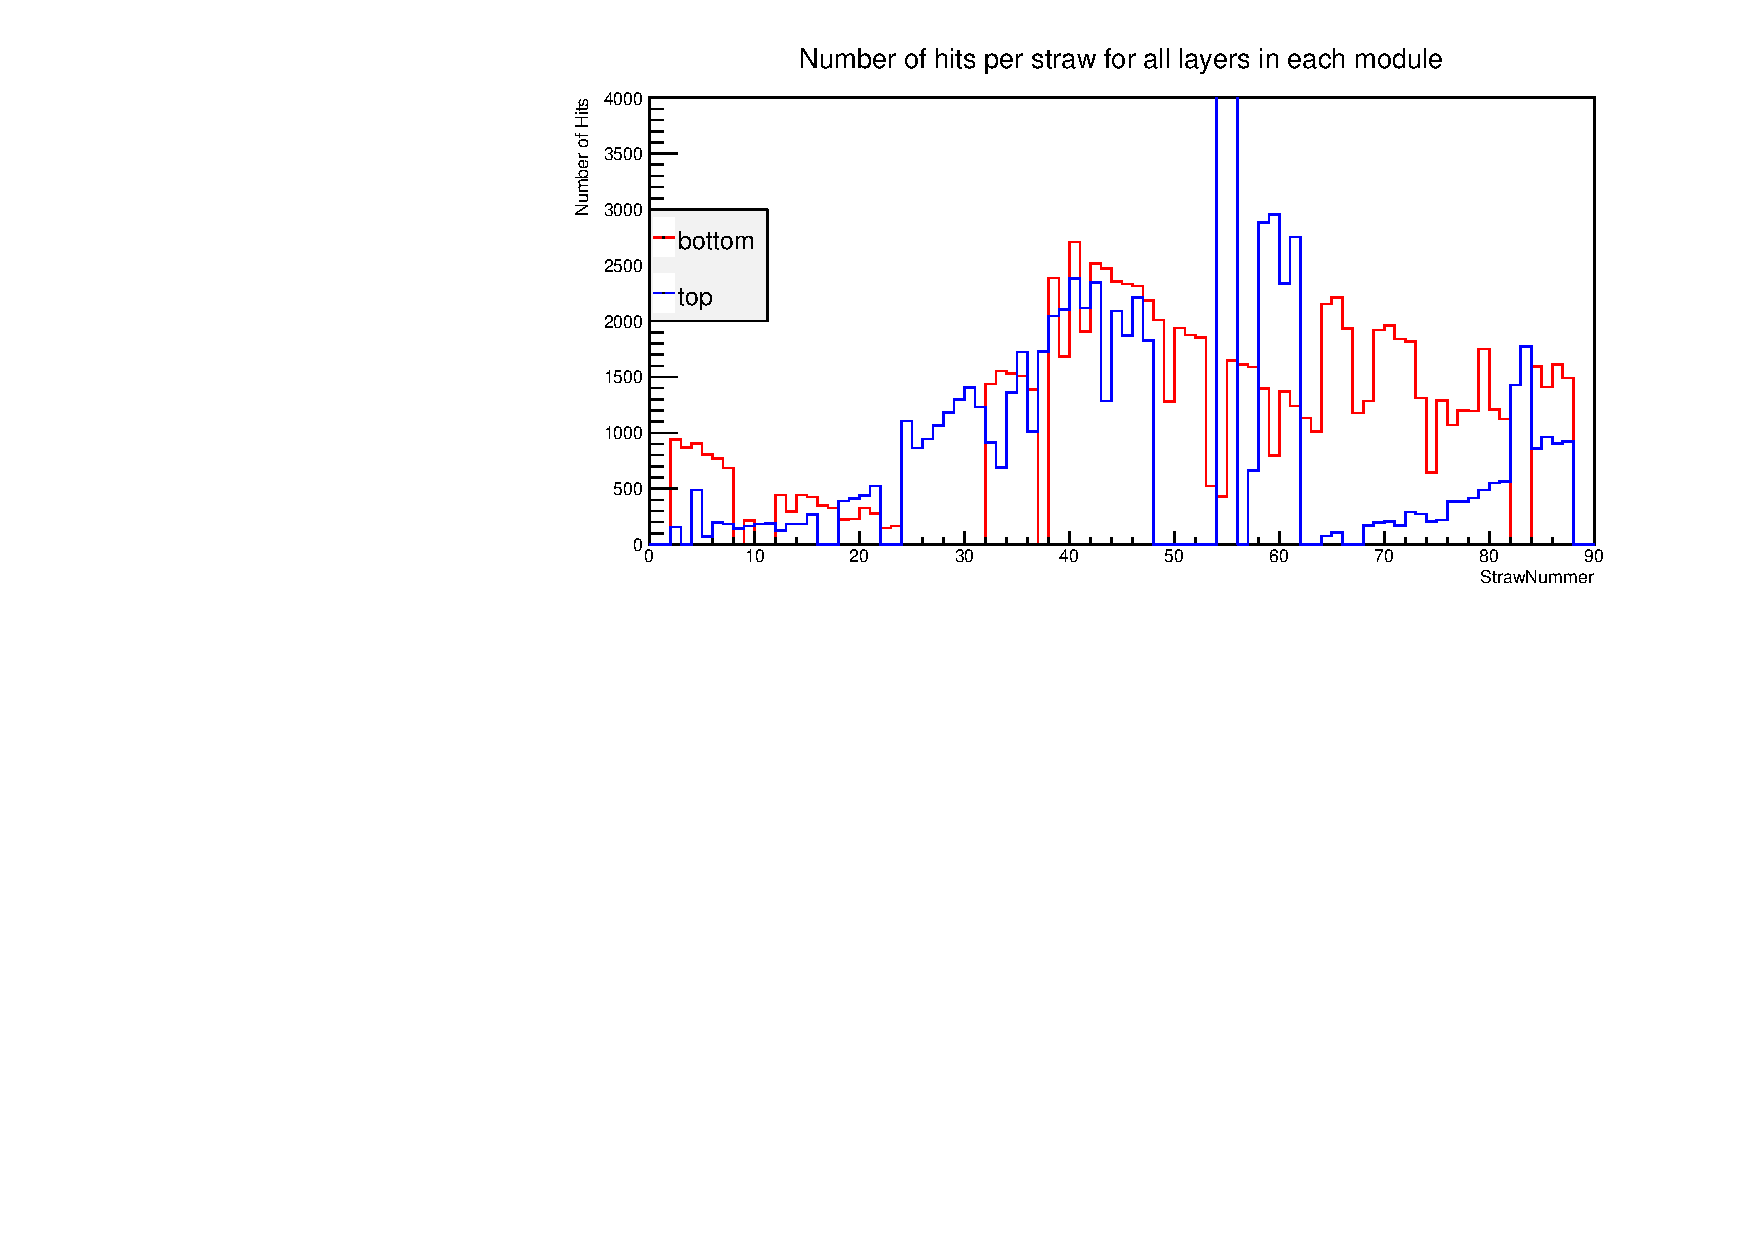
\includegraphics[width=0.8\linewidth]{hitsModules}
	\caption{Number of hits per straws for all layers in bottom and top module}
	\label{fig:hitsModules}
\end{figure}

Figure~\ref{fig:NTrakcs_vs_NHits} shows the correlation between number of tracks and number of hits of an event. According to~\cite{root-bins}, lower limit of a bin is included and upper limit is excluded (it becomes lower limit for the next bin). 

\begin{figure}[ht]
	\centering
	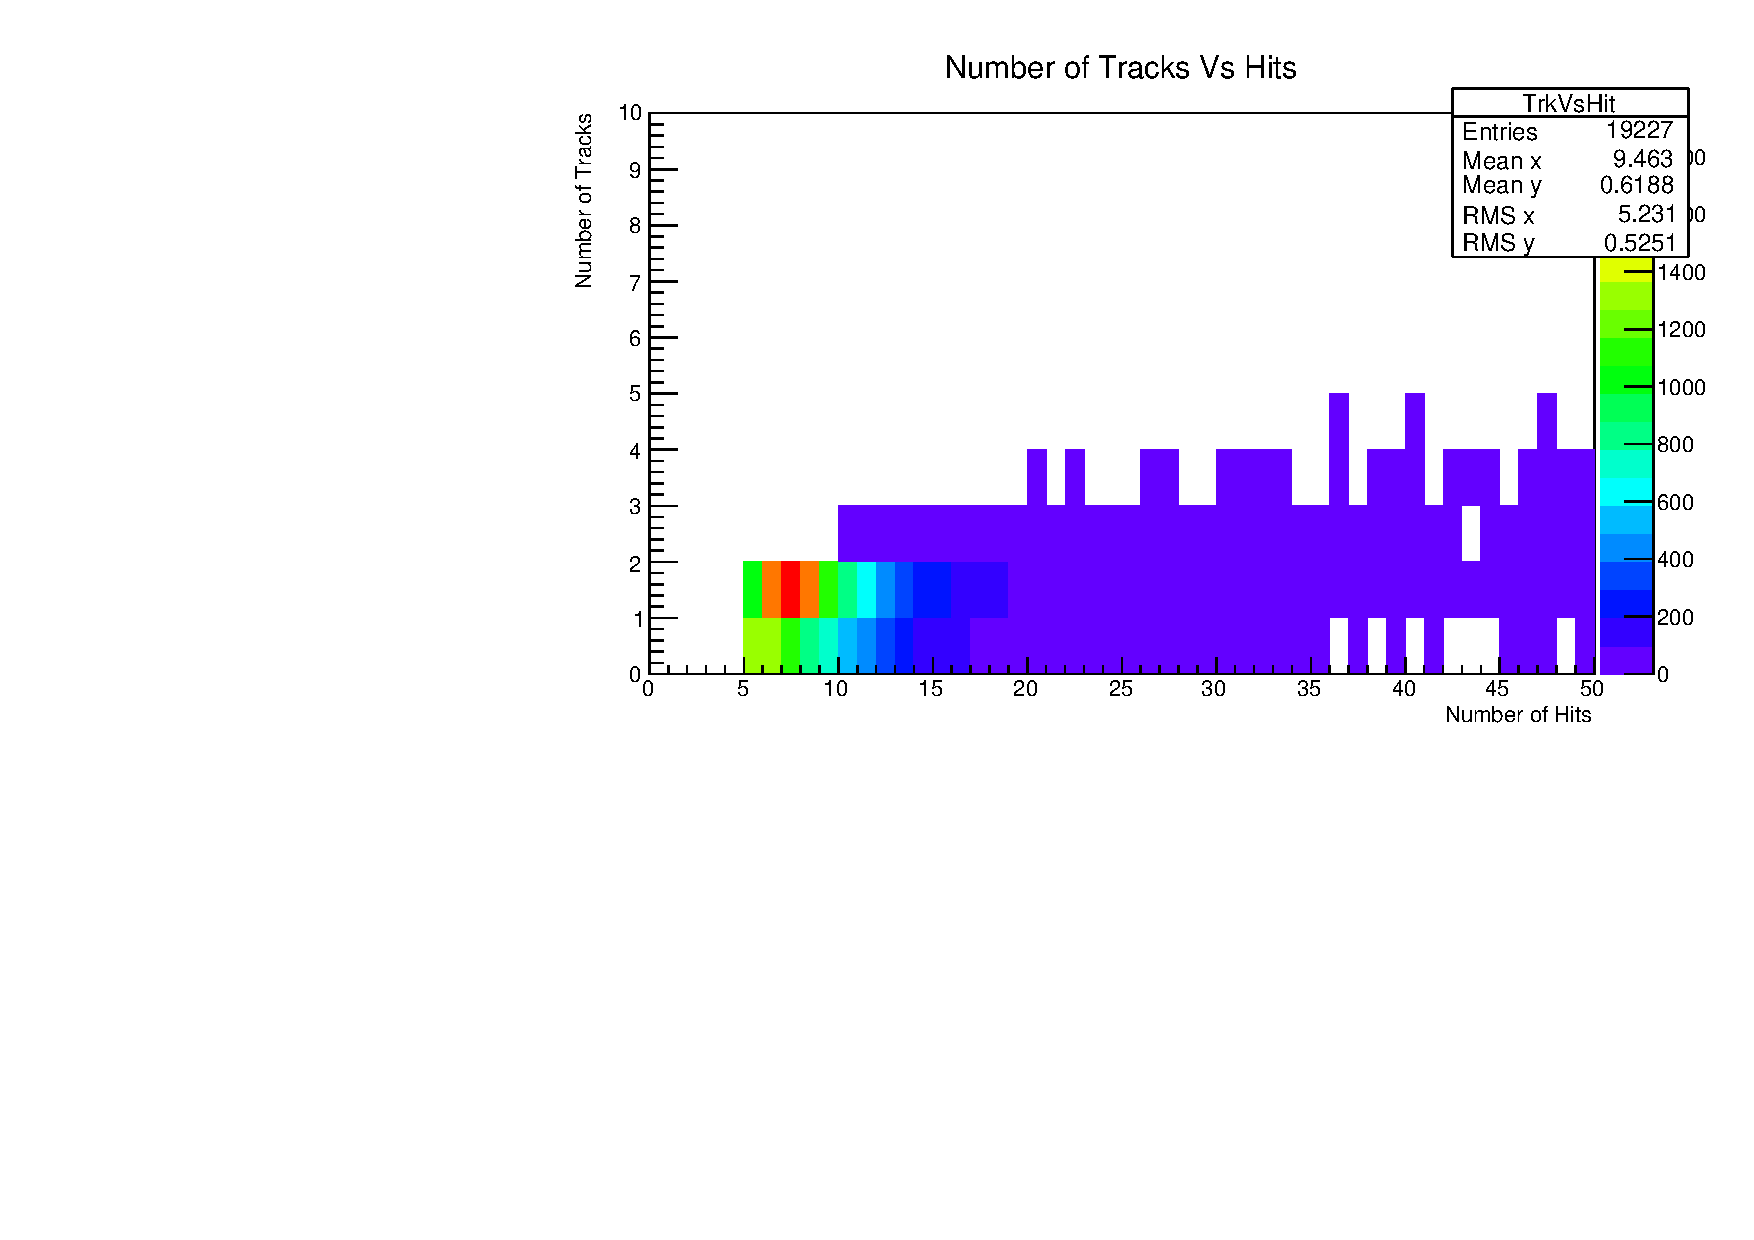
\includegraphics[width=0.8\linewidth]{NTrakcs_vs_NHits.pdf}
	\caption{Number of tracks against number of hits}%
	\label{fig:NTrakcs_vs_NHits}
\end{figure}
There are two clear sharp edges with number of hits at $5$ and $10$ and a couple of more subtle ones with number of hits at $20$ and $\sim 35$. Thus the interpretation of the plot in figure~\ref{fig:NTrakcs_vs_NHits} is that the reconstruction algorithm probably demand minimal $5$ hits for every track. This "rule" breaks down at high number of hits, probably because that an event with high number of tracks is not very likely.

A obvious "hot" region in figure~\ref{fig:NTrakcs_vs_NHits} has number of tracks at $1$ and number of hits $\sim 7$. Thus most events have only $1$ track and $\sim 7$ hits registered. One can try to imagine the distribution projected to horizontal axis, i.e.~an one-dimensional histogram of number of hits. It resembles a shape of Poisson distribution (with a lower cutoff of course), which is characteristic for a counting experiment.

Angular (zenith angle) distribution of events with one track is shown in figure~\ref{fig:angDistri}. It (presumably) is because of limitation of the reconstruction program that only one zenith angle can be stored for one event. This cut will not in theory create a bias in the angular distribution, since there is no reason to believe that multiple tracks in one events are correlated in any way. There is an ambiguity in the data, namely the definition of \verb|track slope| used in the program. We interpreted it as the plain slope instead of the angle, so that the zenith angle is calculated with $\arctan$ function. Either way, the "choice" of the definition has virtually no impact on the angular distribution and following fit.

\begin{figure}[ht]
	\centering
	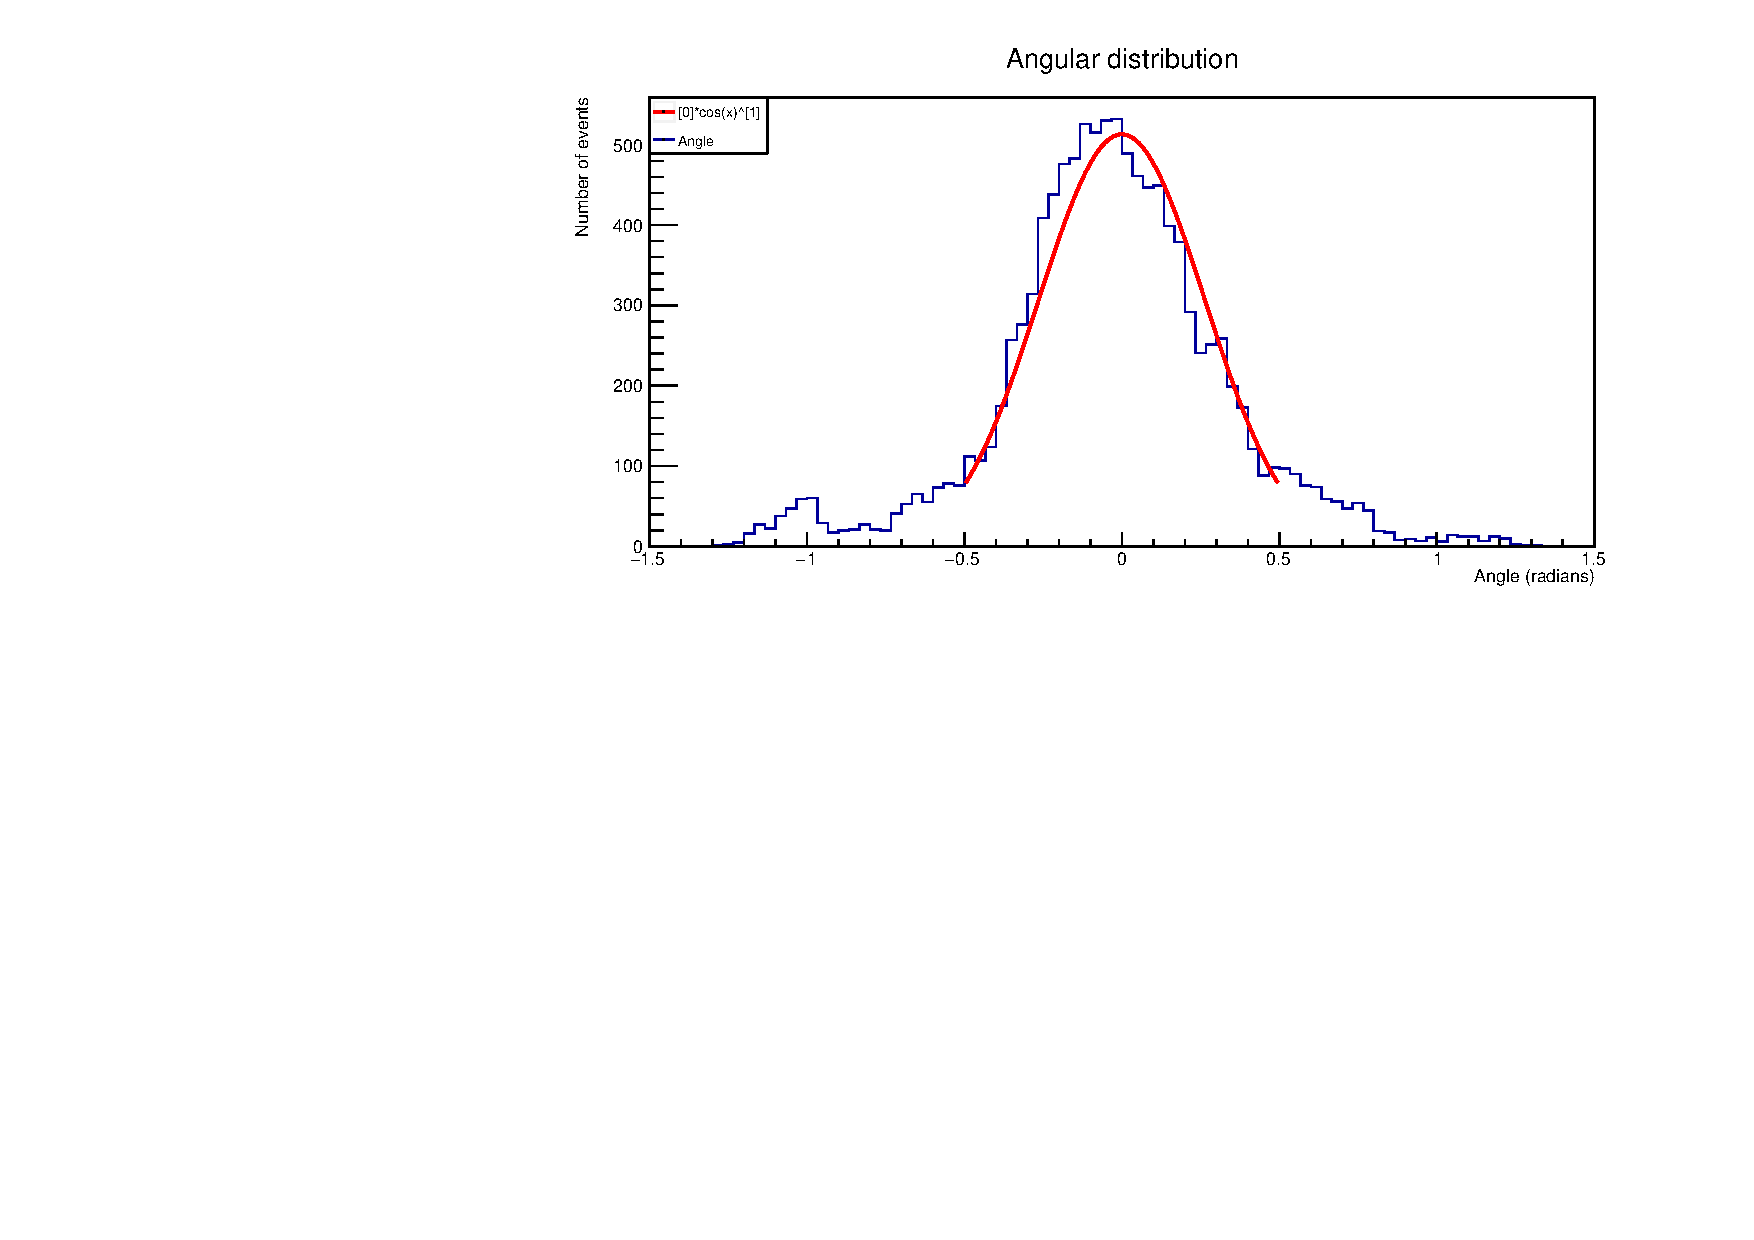
\includegraphics[width=0.8\linewidth]{angDistri.pdf}
	\caption{Angular distribution of events with a single track}%
	\label{fig:angDistri}
\end{figure}
Basic features of figure~\ref{fig:angDistri} are sort of expected. It peaks at zero zenith angle, since decay probability starts to increase with the angle, see equation~\ref{math:cos2}. A closer look reveals that the histogram is as we expect. A fit is done
\begin{equation*}
	f(x) = A  \cos^n x
\end{equation*}
between $\theta=-0.5$ and $\theta=0.5$, since at large angle the $\cos^2$ doesn't apply anymore. $A$ and $n$ are the fit parameters, which are determined as
\begin{align*}
	A &= \num{513.00 +- 6.95} \\
	n &= \num{14.59 +- 0.35} 
\end{align*}
The interval of zenith angle can certainly be adjusted to influence the quality of the fit. But we reckon that our choice should cover the region that distribution is supposed to follow equation~\ref{math:cos2} and some changes don't really affect results too much anyway.

\begin{figure}[H]
	\centering
	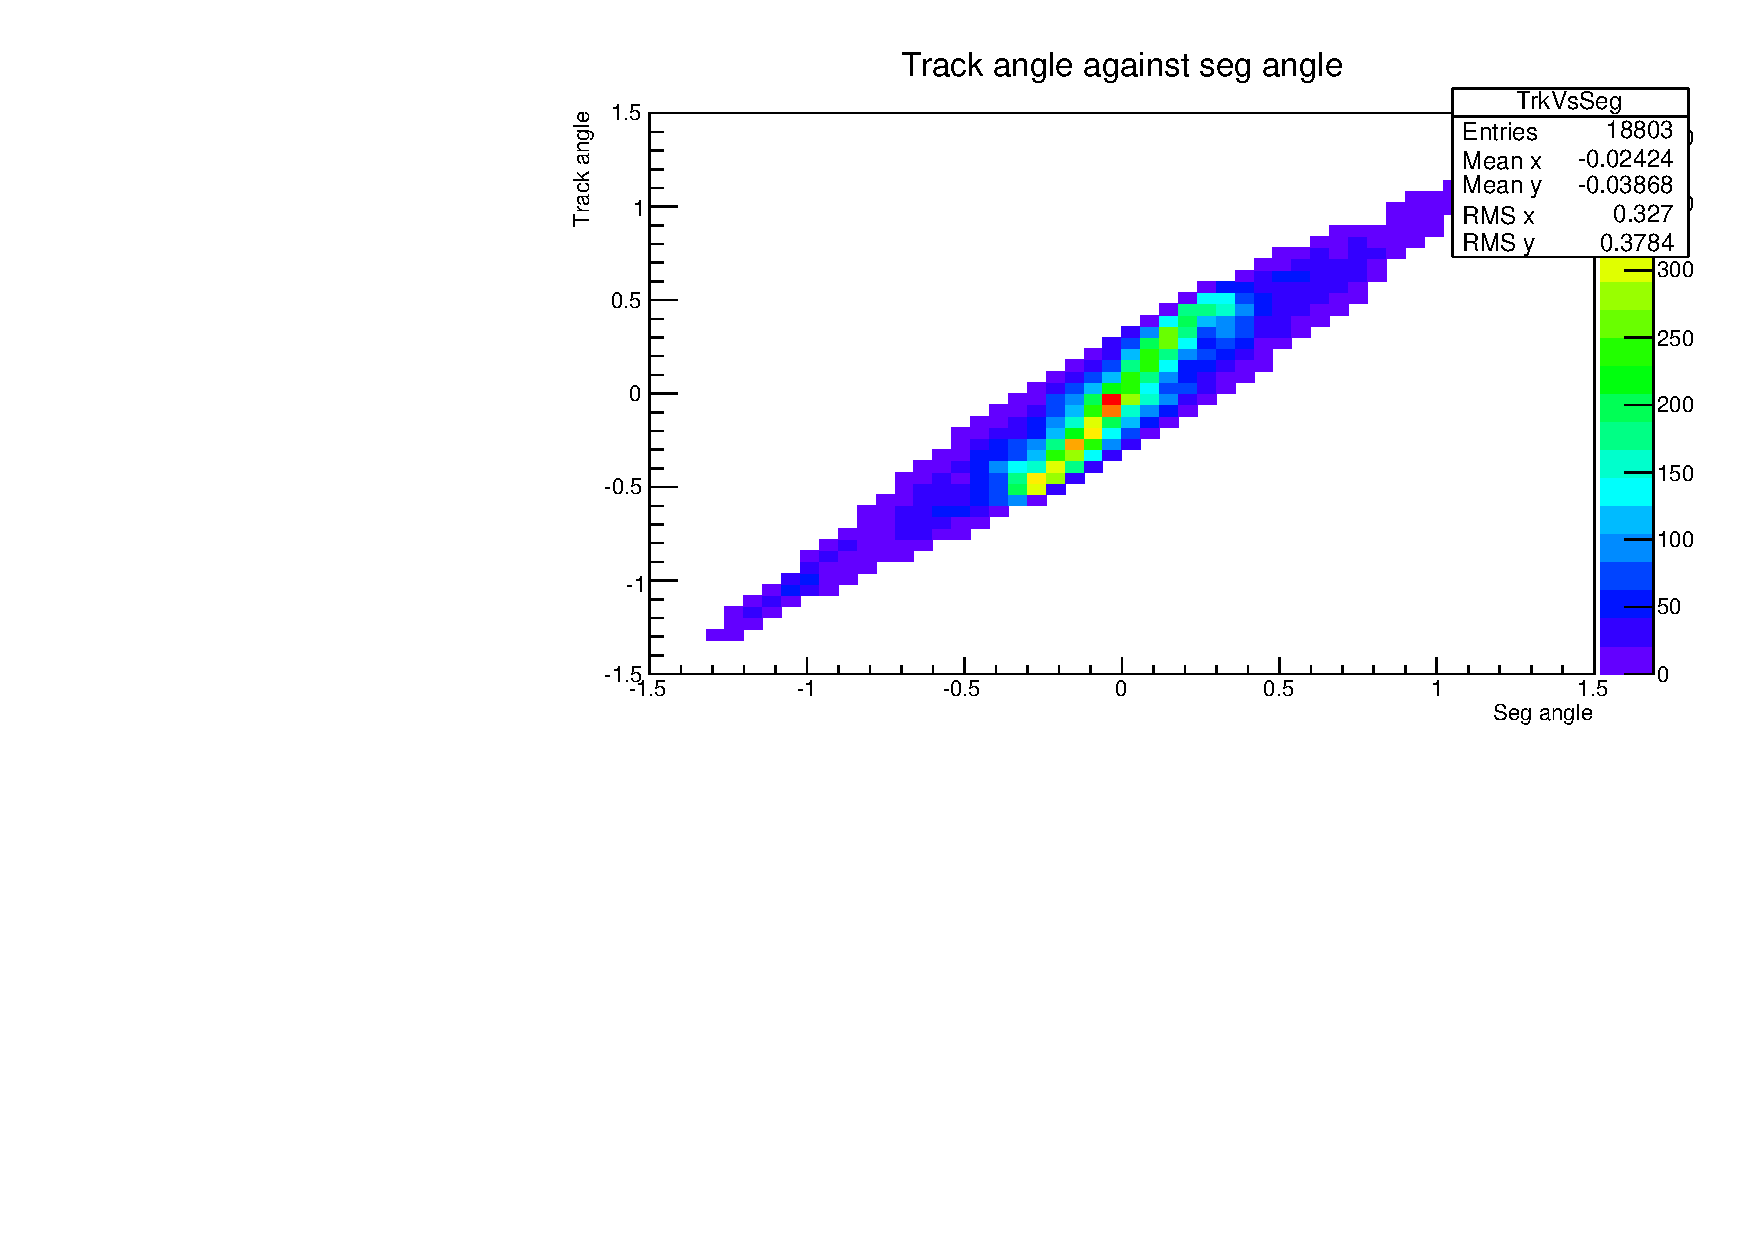
\includegraphics[width=0.8\linewidth]{TracksVsSeg.pdf}
	\caption{Zenith (track) angle against segment angle.}%
	\label{fig:TracksVsSeg}
\end{figure}
Another plot worth investigating is zenith angle (track angle) against segment angle for events with one track, see figure~\ref{fig:TracksVsSeg}. Segment angle, we suppose, denotes the angle of the "track" in only one module. In theory they should match perfectly. But we need to consider detector space/angle resolution, so that the distribution is smeared. Figure~\ref{fig:TracksVsSeg} is almost what we want to see, except the central "hot" regions is inclined a bit and thus the plot is not symmetric along $\ang{45}$ line.

